\documentclass[12pt]{article}

\usepackage{template/sbc-template}
\usepackage{graphicx}
\usepackage{url}
\usepackage[utf8]{inputenc}
\usepackage[T1]{fontenc}
\usepackage[brazil]{babel}

\usepackage{amsmath,amssymb,amsfonts}
\usepackage{booktabs}
\usepackage{multirow}
\usepackage{array}
\usepackage{enumitem}

% Permite que URLs longas quebrem de linha (sem perder o link)
\Urlmuskip=0mu plus 1mu\relax
\makeatletter
\g@addto@macro\UrlBreaks{\do\/\do\-\do\.\do\_\do\?\do\&\do\=\do\#\do\:}
\makeatother

\sloppy

\title{Predição Espaço-Temporal de Acidentes de Trânsito em Rodovias
Federais de Minas Gerais com Graph Neural Networks e Representação
Estrutural da Malha Viária}

\author{
Giovanni Willik Del Piccolo\inst{1},
João Victor De Pascale Souza\inst{2},
Lion Chen\inst{3}
}

\address{
Universidade de São Paulo (USP)\\
São Paulo -- SP -- Brasil\\
\email{\{15455979\inst{1},15463888\inst{2},15470010\inst{3}\}}
}

\newcommand{\pp}{\,p.p.}

\begin{document}

\maketitle

% ============================================================
\begin{abstract}
Traffic accidents on federal highways are a relevant public health
and road-planning problem. This work evaluates whether explicit road
network connectivity improves weekly accident prediction on federal
highways in Minas Gerais, Brazil. Eight annual Federal Highway Police
(PRF) files from 2019 to July 2026 were integrated with a historical
OpenStreetMap network from December 2018. The resulting graph contains
10,973 physical road segments, and 66,186 valid occurrences were
matched within 500 metres. Random Forest, XGBoost, MLP, GraphSAGE and
GATv2 were evaluated with five random seeds and temporal splits:
2019--2023 for training, 2024 for validation, 2025 for the main test
and partial 2026 for an additional test. XGBoost achieved the highest
mean average precision: 0.1675 in 2025 and 0.1723 in 2026. The graph
models did not outperform the tabular baselines. Topology increased
GraphSAGE average precision by 0.0060, but reduced GATv2 performance by
0.0333. A local replay reconstructed the data and repeated inference
with zero metric difference. Results remain conditional on assumed
temporal coverage, a static road network and a limited training
budget.
\end{abstract}

\begin{resumo}
Acidentes em rodovias federais constituem um problema relevante de
saúde pública e planejamento viário. Este trabalho avalia se a
conectividade explícita da malha melhora a predição semanal de
acidentes em rodovias federais de Minas Gerais. Foram integrados oito
arquivos anuais da Polícia Rodoviária Federal (PRF), de 2019 a julho de
2026, e uma malha histórica do OpenStreetMap de dezembro de 2018. O
grafo resultante contém 10.973 segmentos físicos, e 66.186 ocorrências
válidas foram associadas em até 500 metros. Random Forest, XGBoost,
MLP, GraphSAGE e GATv2 foram avaliados com cinco sementes e divisão
temporal: 2019--2023 para treino, 2024 para validação, 2025 para teste
principal e 2026 parcial para teste adicional. XGBoost obteve a maior
precisão média (AP): 0,1675 em 2025 e 0,1723 em 2026. Os modelos em
grafo não superaram as referências tabulares. A topologia elevou a AP
do GraphSAGE em 0,0060, mas reduziu a do GATv2 em 0,0333. A reprodução
local reconstruiu os dados e repetiu as inferências sem diferença nas
métricas. Os resultados são condicionados à cobertura temporal
assumida, à malha estática e ao orçamento limitado de treinamento.
\end{resumo}

% ============================================================
\section{Introdução}
\label{sec:introducao}

Os acidentes de trânsito permanecem entre as principais causas
evitáveis de morte e incapacidade no mundo. O relatório global da
Organização Mundial da Saúde estima aproximadamente 1,19 milhão de
mortes anuais no trânsito e destaca que os impactos recaem de forma
desproporcional sobre países de renda baixa e média
\cite{who2023}. No Brasil, as rodovias federais possuem papel
estratégico na circulação de pessoas e mercadorias e, simultaneamente,
concentram ocorrências com custos humanos, sociais e econômicos. Em
2025, a Polícia Rodoviária Federal registrou 72.483 sinistros e 6.044
mortes nessas vias \cite{prf2026}. Antecipar onde e quando o risco de
uma ocorrência registrada é maior pode apoiar a priorização de
fiscalização, inspeções e análises de engenharia, desde que as
predições sejam interpretadas como suporte analítico, e não como
estimativas causais ou alertas operacionais já validados.

Os dados abertos da PRF permitem investigar o problema em escala
nacional e com localização geográfica. Entretanto, registros de
acidentes não são observações independentes no espaço: segmentos
conectados compartilham fluxos, características construtivas e
continuidade de trajetos. Modelos tabulares convencionais representam
cada trecho apenas por seus atributos, enquanto uma representação em
grafo pode propagar informação entre trechos vizinhos. Essa diferença
motiva a pergunta central deste estudo: \textit{a estrutura de
adjacência da malha viária melhora a predição semanal de acidentes em
rodovias federais de Minas Gerais quando os modelos são avaliados sob a
mesma população, os mesmos atributos não topológicos e a mesma divisão
temporal?}

Trabalhos brasileiros anteriores exploraram os dados da PRF por meio
de regras de associação \cite{araujo2022} e de classificadores de
\textit{hotspots} \cite{amorim2023}. Em paralelo, estudos
internacionais demonstraram o potencial de Graph Neural Networks
(GNNs) para modelar dependências espaciais na segurança viária
\cite{nippani2023,zhang2026,zhuang2024}. Ainda assim, permanecem
diferenças importantes de contexto, fontes, unidade de análise e
protocolo. Resultados obtidos em redes norte-americanas ou europeias
não estabelecem, por si só, que a topologia será útil em rodovias
brasileiras, sobretudo quando dados de tráfego, imagens de satélite ou
históricos publicados antes da previsão não estão disponíveis.

Para responder à pergunta, o projeto construiu uma base auditável que
combina ocorrências da PRF de 2019 a julho de 2026 com uma malha
histórica do OpenStreetMap (OSM). A unidade analítica é o par
segmento--semana, e o alvo indica se houve ao menos uma ocorrência
registrada no segmento durante uma semana completa. O desenho
experimental separa cronologicamente 2019--2023 para treinamento, 2024
para validação e definição de limiares, 2025 para teste principal e
2026 parcial para teste temporal adicional. A comparação inclui três
modelos sem acesso à vizinhança explícita --- Random Forest, XGBoost e
uma rede neural multicamadas (MLP) --- e duas GNNs --- GraphSAGE e
GATv2. Todos foram executados com cinco sementes; GraphSAGE e GATv2
também receberam ablações de atributos viários, atributos temporais e
topologia.

As contribuições do trabalho são quatro. Primeiro, foi implementado um
\textit{pipeline} reproduzível de aquisição, curadoria, associação
espacial e formação de alvos semanais, com auditoria das exclusões e
controle de vazamento temporal. Segundo, foi construída uma
representação de 10.973 segmentos federais mineiros como nós de um
grafo, preservando componentes desconectados e pistas paralelas.
Terceiro, cinco famílias de modelos foram comparadas na mesma
população e em dois períodos posteriores ao desenvolvimento. Quarto,
as ablações permitiram separar, de forma descritiva, o efeito observado
dos atributos de via, do calendário e da passagem de mensagens.

O resultado principal é negativo em relação à hipótese mais forte:
nenhuma GNN superou os modelos tabulares em AP. XGBoost liderou os dois
testes, enquanto a topologia apresentou efeito dependente da
arquitetura: pequeno ganho para GraphSAGE e perda para GATv2. Esse
achado não invalida GNNs de forma geral; delimita o que foi observado
com esta base, este orçamento e estas configurações. As seções
seguintes apresentam os trabalhos correlatos, a metodologia, os
resultados e suas limitações.

% ============================================================
% Trabalhos correlatos: máximo de três páginas
% ============================================================
\section{Trabalhos Relacionados}
\label{sec:correlatos}

\subsection{Estudos com dados brasileiros}

Araújo \cite{araujo2022} investigou dados nacionais da PRF entre
janeiro de 2017 e fevereiro de 2020, enriquecidos com atributos de
veículos do RENAVAM. Apriori, Eclat, FP-Growth e FP-Max foram usados
para identificar regras entre causas, veículos, vias, usuários e
ambiente. O estudo demonstrou a riqueza da base para mineração de
padrões e observou comportamento distinto do FP-Max em regras mais
extensas. Sua tarefa, porém, é descritiva: suporte e confiança de
regras não medem capacidade de prever ocorrências futuras. Além disso,
a conectividade entre segmentos não integra o modelo.

Amorim et al. \cite{amorim2023} aplicaram SVM, Random Forest e MLP à
classificação de \textit{hotspots} de rodovias federais brasileiras
como severos ou não severos. A MLP apresentou acurácia de 83\% e F1 de
82\%. O trabalho confirma a viabilidade de aprendizado supervisionado
com dados da PRF, mas a população é formada por \textit{hotspots} e o
alvo é severidade. No presente estudo, todas as unidades
segmento--semana elegíveis são avaliadas, inclusive as sem ocorrência,
e o alvo é a presença de acidente. Por isso, comparações numéricas
diretas entre as métricas não representam um \textit{benchmark}
equivalente.

\subsection{GNNs para segurança viária}

Nippani et al. \cite{nippani2023} construíram um \textit{benchmark} de
GNNs para contagem e ocorrência de acidentes em redes viárias dos
Estados Unidos. Modelos como GraphSAGE alcançaram AUROC acima de 87\%
na classificação e erro absoluto médio relativo abaixo de 22\% na
contagem, sustentando que relações topológicas podem acrescentar
informação. O estudo motivou a escolha do GraphSAGE, mas utiliza outra
rede, outras fontes e outra exposição ao tráfego.

Zhang et al. \cite{zhang2026} combinaram grafo, imagens de satélite,
clima, tipo de via e volume de tráfego em aproximadamente nove milhões
de registros de seis estados norte-americanos. A fusão multimodal
atingiu AUROC médio de 90,1\%, ganho de 3,7\pp sobre a variante sem
imagens. O trabalho evidencia o valor de atributos ambientais ricos,
mas depende de modalidades não utilizadas aqui. Este projeto investiga
uma configuração mais restrita e reproduzível com PRF, OSM e
calendário.

Gao et al. \cite{zhuang2024} propuseram uma GNN espaço-temporal
probabilística com distribuição Tweedie inflada de zeros para dados de
Londres. O modelo trata simultaneamente esparsidade, valores extremos e
incerteza. A principal relação com este estudo é o reconhecimento de
que a maioria das unidades espaço-temporais não contém acidentes.
Entretanto, o alvo atual é binário, sem previsão multi-passo de
contagem ou quantificação probabilística de incerteza.

\begin{table}[htbp]
\centering
\caption{Síntese dos trabalhos correlatos e da diferença de escopo.}
\label{tab:correlatos}
\footnotesize
\setlength{\tabcolsep}{3.5pt}
\resizebox{\textwidth}{!}{%
\begin{tabular}{>{\raggedright\arraybackslash}p{2.0cm}
                >{\raggedright\arraybackslash}p{2.3cm}
                >{\raggedright\arraybackslash}p{2.8cm}
                >{\raggedright\arraybackslash}p{5.1cm}
                >{\centering\arraybackslash}p{1.0cm}}
\toprule
\textbf{Trabalho} & \textbf{Contexto} & \textbf{Tarefa e método} &
\textbf{Resultado ou limitação relevante} & \textbf{Grafo} \\
\midrule
Araújo \cite{araujo2022} &
PRF nacional, 2017--2020 &
Regras de associação &
Análise descritiva; não prevê períodos futuros &
Não \\
\addlinespace
Amorim et al. \cite{amorim2023} &
Rodovias federais brasileiras &
Severidade de \textit{hotspots}; SVM, RF e MLP &
MLP com 83\% de acurácia e 82\% de F1; alvo distinto &
Não \\
\addlinespace
Nippani et al. \cite{nippani2023} &
Redes dos Estados Unidos &
Ocorrência e contagem; \textit{benchmark} de GNNs &
AUROC superior a 87\%; contexto e exposição distintos &
Sim \\
\addlinespace
Zhang et al. \cite{zhang2026} &
Seis estados dos Estados Unidos &
GNN multimodal &
AUROC médio de 90,1\%; requer imagens, clima e tráfego &
Sim \\
\addlinespace
Gao et al. \cite{zhuang2024} &
Londres &
GNN probabilística inflada de zeros &
Modela contagem e incerteza; maior complexidade &
Sim \\
\addlinespace
\textbf{Este trabalho} &
Rodovias federais de MG &
Ocorrência por segmento--semana; cinco modelos &
Comparação temporal comum, ablações e reprodução local &
Sim \\
\bottomrule
\end{tabular}%
}
\end{table}

\subsection{Lacuna e posicionamento}

Os estudos brasileiros estabelecem o valor dos dados da PRF, mas não
testam passagem de mensagens em um grafo de segmentos sob avaliação
temporal. Os estudos com GNNs mostram resultados promissores, porém em
outras regiões e, frequentemente, com dados de tráfego ou modalidades
adicionais. A lacuna abordada aqui é, portanto, uma comparação
controlada no contexto mineiro: modelos tabulares e em grafo recebem a
mesma população, os mesmos atributos de via e calendário, e somente as
GNNs recebem adjacência.

O estudo não reproduz diretamente nenhum trabalho correlato e não
pretende estabelecer superioridade entre artigos com tarefas
diferentes. Sua contribuição comparativa é interna: medir se a
topologia melhora os resultados em relação às referências do próprio
experimento. Em relação a Araújo, acrescenta predição temporal e
estrutura espacial; em relação a Amorim, muda o alvo de severidade de
\textit{hotspots} para ocorrência na população completa; em relação
aos trabalhos internacionais, testa GNNs com fontes abertas e
restrições realistas do cenário brasileiro.

% ============================================================
% Metodologia: máximo de três páginas
% ============================================================
\section{Metodologia}
\label{sec:metodologia}

\subsection{Fontes, recorte e curadoria}

Foram utilizados oito arquivos anuais da PRF agrupados por ocorrência,
de 2019 a 2026. O arquivo de 2026 contém registros observados entre 1º
de janeiro e 31 de julho e foi tratado como parcial. A execução adotou,
por autorização do pesquisador, a hipótese de que os arquivos de
2019--2025 cobrem seus anos e o arquivo de 2026 cobre janeiro--julho.
Essa autorização permitiu formar alvos, mas não equivale a comprovação
oficial de completude; possíveis lacunas permanecem uma ameaça à
validade.

A ingestão preservou os arquivos originais, normalizou esquema, datas e
coordenadas e registrou uma decisão de qualidade para cada linha.
Somente registros com \texttt{UF=MG}, coordenadas válidas e posição
compatível com o estado seguiram para a associação espacial.
Duplicidades e falhas não foram corrigidas silenciosamente. A
validade intrínseca do registro foi mantida separada da elegibilidade
da semana como alvo.

A malha federal foi obtida do OSM em uma extração histórica com
referência em 31 de dezembro de 2018, evitando que vias posteriores ao
início do estudo fossem incorporadas automaticamente. Segmentos foram
recortados ao interior de Minas Gerais. Arestas recíprocas com a mesma
geometria foram consolidadas como um segmento físico; pistas paralelas
distintas foram preservadas.

\subsection{Grafo, associação espacial e unidade analítica}

Na rede viária original, interseções são nós e trechos são arestas.
Para as GNNs foi construído o grafo de linhas: cada segmento físico
torna-se um nó, e dois nós são adjacentes quando os segmentos
compartilham uma junção OSM. Cruzamentos apenas geométricos não criam
conexões. Pares repetidos foram removidos antes da passagem de
mensagens; segmentos isolados e componentes desconectados foram
preservados.

Cada ocorrência foi projetada com a malha no sistema EPSG:5880 e
associada ao segmento elegível mais próximo. Distâncias de até 500
metros, inclusive, foram aceitas; empates foram resolvidos por
identificador canônico. A distância e o motivo de rejeição foram
armazenados para auditoria.

As observações foram formadas para todas as combinações entre 10.973
segmentos e semanas civis completas. Semanas que cruzam partições,
ultrapassam o corte da fonte ou não possuem sete dias cobertos foram
excluídas. Múltiplas ocorrências no mesmo segmento e semana resultam em
um único alvo positivo.

\subsection{Atributos e pré-processamento}

Os atributos viários são comprimento, tipo de via, número de faixas,
velocidade máxima, sinuosidade e indicadores de ausência. Os atributos
temporais incluem ano, mês, semana ISO, seno e cosseno da semana. Foram
previstas contagens defasadas de 1, 4, 13 e 52 semanas e o número de
semanas históricas disponíveis. Contudo, a publicação anterior dos
registros não foi comprovada; por integridade temporal, esses históricos
permaneceram ausentes, com indicadores explícitos. Assim, a ablação
temporal avalia principalmente o calendário.

O pré-processador comum foi ajustado apenas em 2019--2023. Variáveis
numéricas receberam imputação pela mediana, indicadores adicionais de
ausência e padronização; o tipo de via recebeu imputação para categoria
desconhecida e codificação \textit{one-hot}. O transformador congelado
foi reutilizado em validação e testes.

\subsection{Modelos e protocolo experimental}

O Random Forest \cite{breiman2001} utilizou 50 árvores, profundidade
máxima 12, mínimo de cinco amostras por folha e subconjunto de atributos
pela raiz quadrada. O XGBoost \cite{chen2016} utilizou 100 árvores,
profundidade 6, taxa de aprendizado 0,05, subamostragem de 0,8 e
amostragem de colunas de 0,8. MLP \cite{goodfellow2016}, GraphSAGE
\cite{hamilton2017} e GATv2 \cite{brody2022} possuem uma camada oculta
de 64 unidades, \textit{dropout} 0,1, Adam com taxa $10^{-3}$ e
decaimento $10^{-4}$, treinados por cinco épocas. O GATv2 usa duas
cabeças de atenção na primeira camada.
O orçamento foi definido antes dos testes e contém um candidato por
família ou variante; não representa busca exaustiva nem garantia de
convergência.

A ponderação das classes foi calculada somente no treinamento:
\texttt{class\_weight=balanced} no Random Forest,
\texttt{scale\_pos\_weight} no XGBoost e perda de entropia cruzada
binária ponderada nas redes.

\begin{table}[htbp]
\centering
\caption{Partições temporais e populações do experimento.}
\label{tab:particoes}
\small
\setlength{\tabcolsep}{5pt}
\begin{tabular}{lrrrr}
\toprule
\textbf{Partição} & \textbf{Semanas} & \textbf{Observações} &
\textbf{Positivos} & \textbf{Prevalência} \\
\midrule
Treino (2019--2023) & 260 & 2.852.980 & 36.837 & 1,29\% \\
Validação (2024) & 52 & 570.596 & 7.918 & 1,39\% \\
Teste (2025) & 51 & 559.623 & 8.092 & 1,45\% \\
Teste (2026 parcial) & 29 & 318.217 & 4.513 & 1,42\% \\
\bottomrule
\end{tabular}
\end{table}

Cada modelo completo foi treinado com as sementes 101, 202, 303, 404
e 505, totalizando 25 execuções. GraphSAGE e GATv2 receberam três
ablações em 2025: sem atributos de via, sem atributos temporais e sem
topologia, acrescentando 30 execuções e totalizando 55 treinamentos.
A variante sem topologia preserva a transformação do próprio nó, mas
remove mensagens de vizinhos.

\subsection{Avaliação, congelamento e reprodução}

A seleção de configurações e a referência tabular foram definidas com
a validação de 2024. Os limiares foram escolhidos pela maximização do
F1 nesse mesmo conjunto. Após o congelamento, os mesmos pesos,
transformadores e limiares foram aplicados aos testes de 2025 e 2026,
sem novo ajuste. AP foi a métrica principal \cite{saito2015}; AUROC, F1,
precisão e revocação foram métricas complementares. Os resultados são
médias e desvios-padrão amostrais entre sementes.

Fontes, configurações, código, modelos, preditores, escores e relatórios
foram identificados por hashes. Um pacote portátil foi criado após a
geração do relatório experimental. A reprodução completa reconstruiu o
conjunto de dados e repetiu as inferências em processo separado, com
rede bloqueada e nenhuma chamada de treinamento. Essa verificação mede
reprodutibilidade computacional local, não replicação externa em outro
ambiente.

\clearpage

% ============================================================
% Resultados e discussão: máximo de seis páginas, com uma página
% adicional admitida para figuras/tabelas.
% ============================================================
\section{Resultados e Discussão dos Resultados}
\label{sec:resultados}

\subsection{Curadoria, associação espacial e estrutura da rede}

Os oito arquivos continham 516.089 registros nacionais. O filtro
inicial identificou 67.065 linhas com indicação de Minas Gerais; após
as validações intrínsecas, 67.023 registros seguiram para associação
espacial. Desses, 66.186 foram associados a um segmento em até 500
metros, taxa global de 98,75\%. As taxas anuais variaram de 97,38\% a
99,17\%, com redução nos arquivos recentes. A mediana da distância
entre ponto e segmento permaneceu próxima de 3,5 metros entre 2019 e
2024, mas aumentou para 6,45 metros em 2025 e 6,76 metros em 2026; o
percentil 95 passou de 22,75 metros em 2024 para 92,93 e 77,71 metros.
Os valores ainda respeitam o corte, mas a cauda maior sugere mudanças
de georreferenciamento ou divergências entre ocorrências recentes e a
malha histórica.

\begin{figure}[htbp]
\centering
\begin{minipage}[c]{0.38\textwidth}
\centering
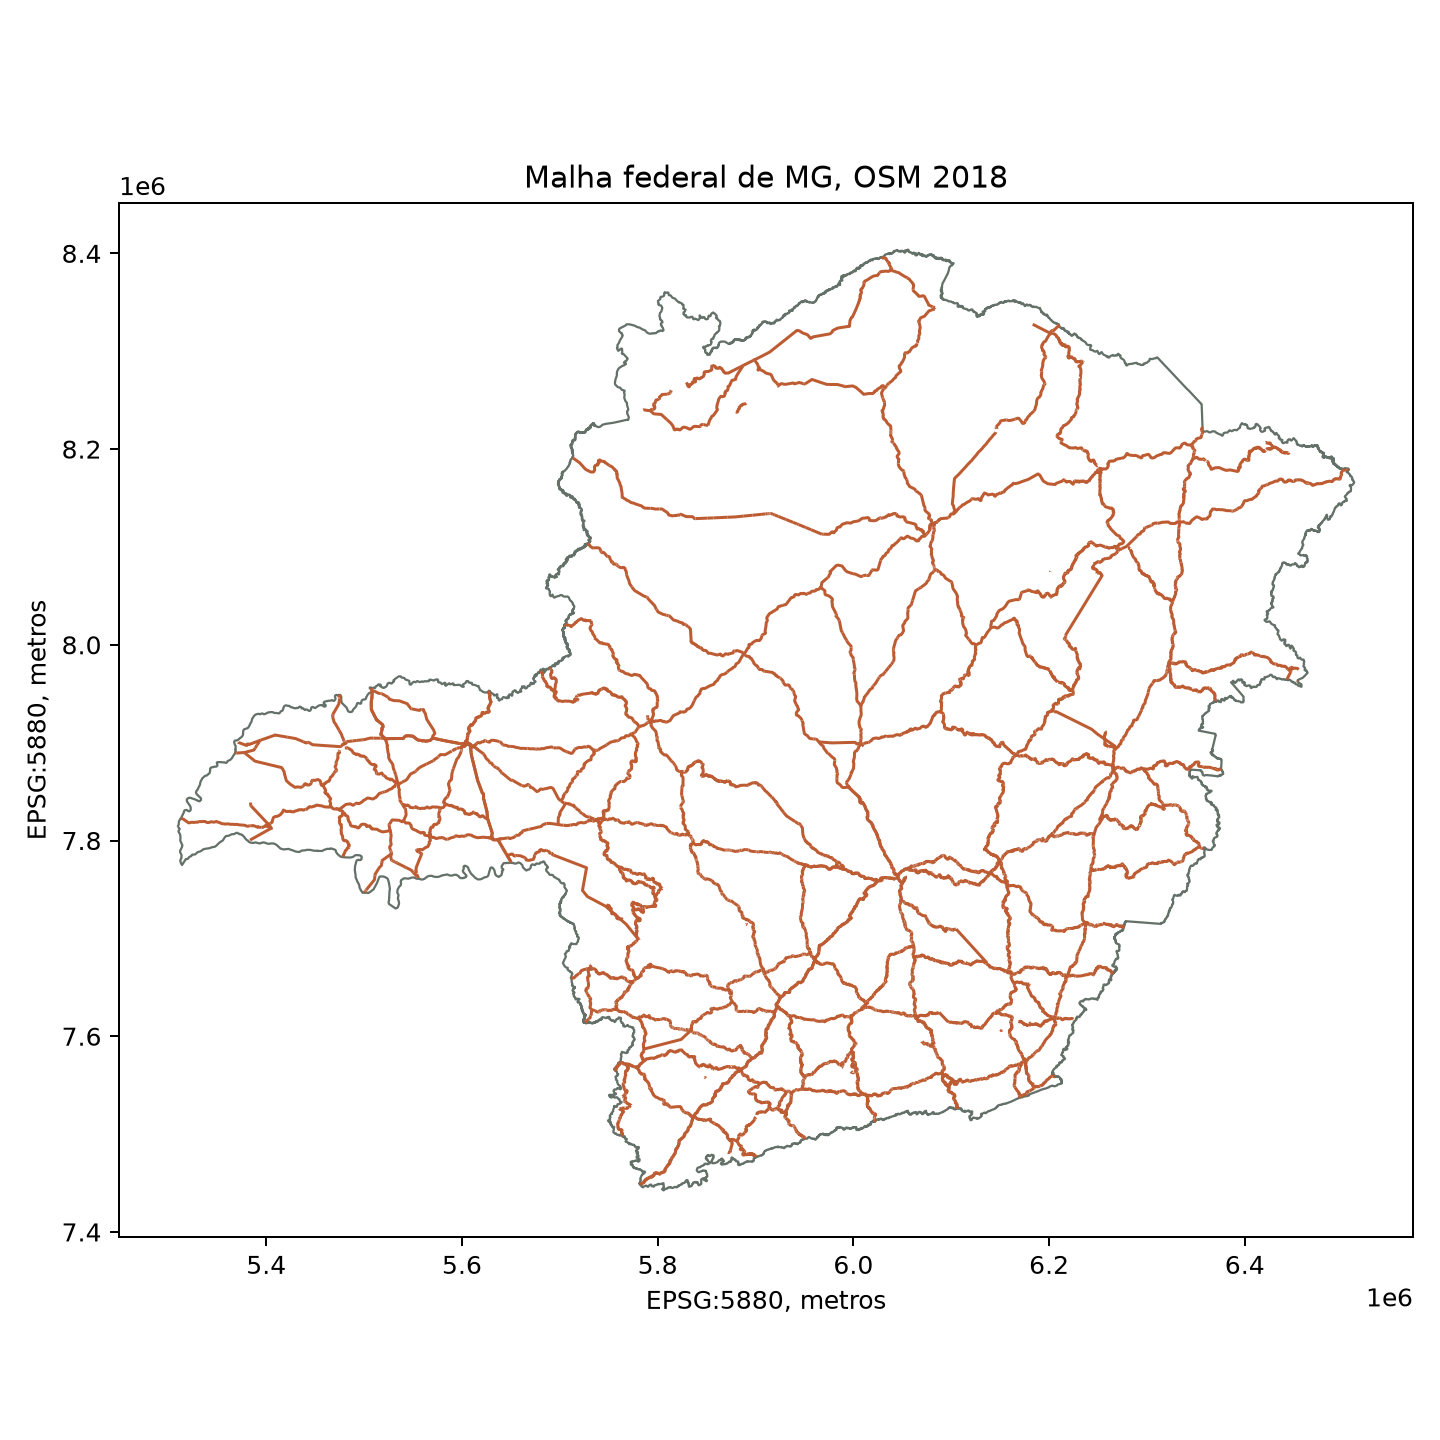
\includegraphics[width=\linewidth]{imagens/historical-federal-map.png}
\end{minipage}\hfill
\begin{minipage}[c]{0.59\textwidth}
\centering
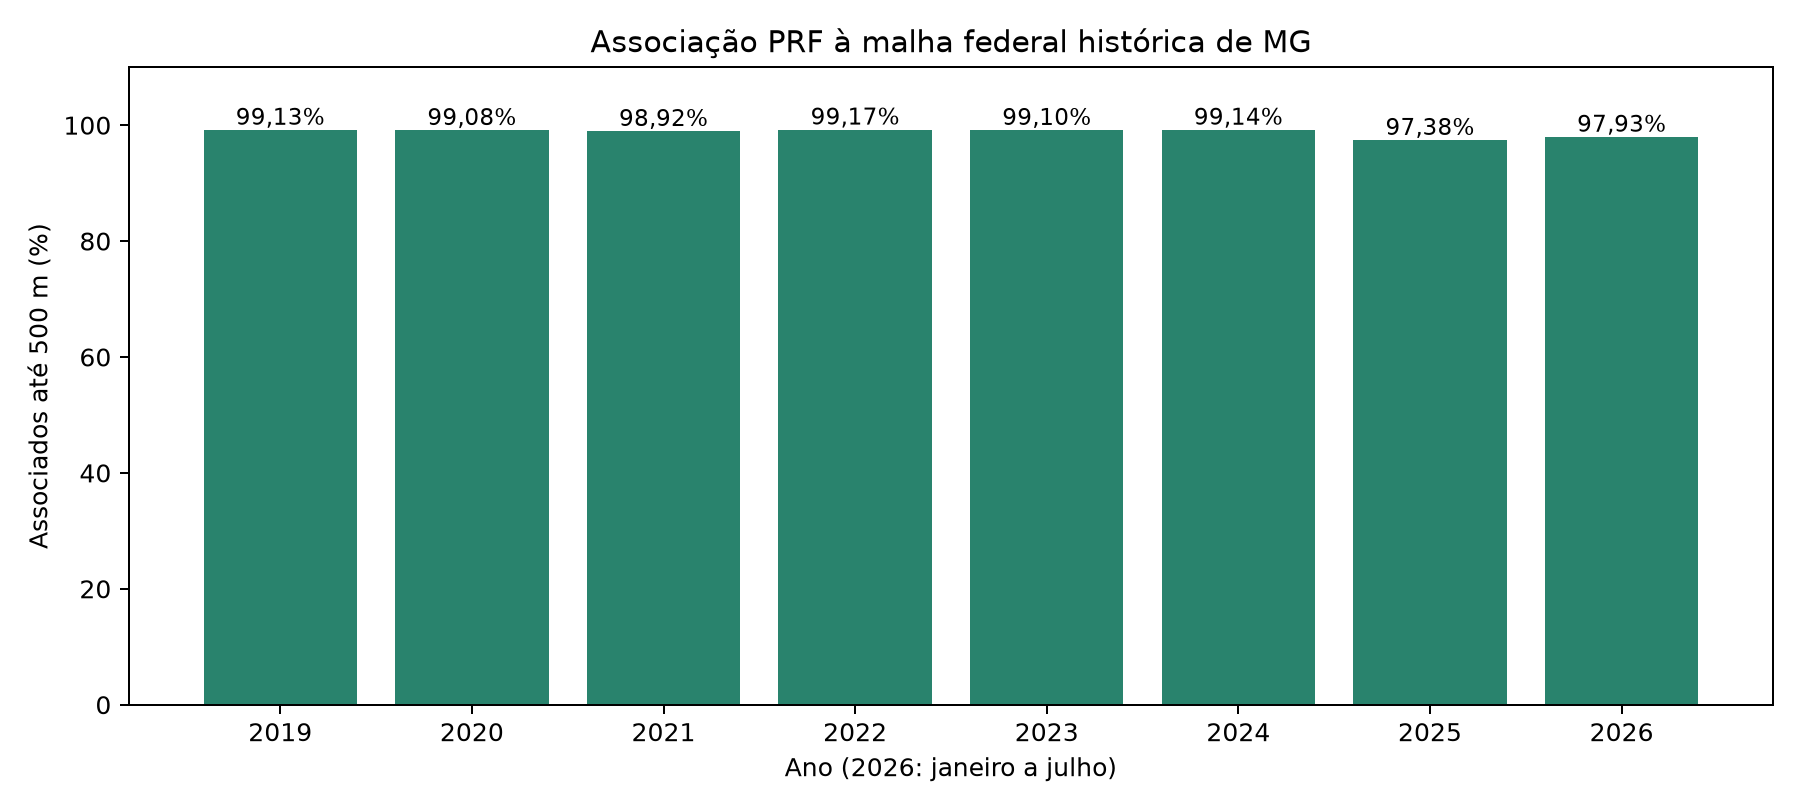
\includegraphics[width=\linewidth]{imagens/federal-snapping.png}
\end{minipage}
\caption{Malha federal histórica de Minas Gerais e percentual anual de
ocorrências associadas em até 500 metros. Fonte: malha e associações
espaciais do conjunto de dados preparado.}
\label{fig:malha-associacao}
\end{figure}

A malha contém 10.973 segmentos físicos, 14.636 pares únicos de
segmentos adjacentes e 92 componentes conexos. O maior componente reúne
9.782 segmentos e 30 segmentos são isolados. A soma das geometrias é
19.607,9 km, valor que não equivale à extensão oficial porque pistas
paralelas contribuem separadamente. Também há lacunas relevantes:
6.187 segmentos não possuem número de faixas e 6.955 não possuem
velocidade máxima. Essas ausências foram modeladas como informação
faltante, e não como zero.

Ao todo, 65.536 ocorrências associadas pertencem a semanas elegíveis
nas quatro partições. Elas geraram 57.360 unidades positivas entre
4.301.416 pares segmento--semana. A prevalência variou pouco, de 1,29\%
no treino a 1,45\% em 2025, confirmando o forte desbalanceamento. Os
negativos representam ausência de registro sob a hipótese de cobertura
declarada, não prova de que nenhum acidente ocorreu.

\subsection{Desempenho dos cinco modelos}

A Tabela~\ref{tab:desempenho} apresenta os modelos completos. XGBoost
alcançou a maior AP e a maior AUROC nos dois testes. Em 2025, sua AP de
16,75\% corresponde a aproximadamente 11,6 vezes a prevalência de
1,45\%; em 2026, a AP de 17,23\% corresponde a aproximadamente 12,1
vezes a prevalência de 1,42\%. Random Forest e MLP ficaram próximos do
XGBoost, enquanto GraphSAGE e GATv2 apresentaram menor capacidade de
ordenar a classe positiva.

\begin{table}[htbp]
\centering
\caption{Desempenho médio dos modelos completos. Valores em porcentagem,
com desvio-padrão amostral entre cinco sementes.}
\label{tab:desempenho}
\footnotesize
\setlength{\tabcolsep}{3.2pt}
\resizebox{\textwidth}{!}{%
\begin{tabular}{lcccccc}
\toprule
\multirow{2}{*}{\textbf{Modelo}} &
\multicolumn{3}{c}{\textbf{Teste 2025}} &
\multicolumn{3}{c}{\textbf{Teste 2026 parcial}} \\
\cmidrule(lr){2-4}\cmidrule(lr){5-7}
& \textbf{AP} & \textbf{AUROC} & \textbf{F1}
& \textbf{AP} & \textbf{AUROC} & \textbf{F1} \\
\midrule
Random Forest &
$16{,}12\pm0{,}22$ & $92{,}19\pm0{,}02$ & $24{,}86\pm0{,}12$ &
$16{,}58\pm0{,}26$ & $91{,}98\pm0{,}04$ & $24{,}77\pm0{,}13$ \\
XGBoost &
$16{,}75\pm0{,}18$ & $92{,}28\pm0{,}03$ & $24{,}73\pm0{,}42$ &
$17{,}23\pm0{,}20$ & $92{,}10\pm0{,}03$ & $24{,}84\pm0{,}21$ \\
MLP &
$16{,}24\pm0{,}08$ & $91{,}70\pm0{,}01$ & $24{,}60\pm0{,}13$ &
$16{,}53\pm0{,}14$ & $91{,}72\pm0{,}05$ & $24{,}71\pm0{,}23$ \\
GraphSAGE &
$13{,}86\pm0{,}48$ & $90{,}39\pm0{,}13$ & $22{,}14\pm0{,}34$ &
$13{,}90\pm0{,}46$ & $90{,}50\pm0{,}14$ & $22{,}68\pm0{,}37$ \\
GATv2 &
$10{,}37\pm0{,}49$ & $87{,}31\pm0{,}37$ & $18{,}25\pm0{,}74$ &
$10{,}82\pm0{,}58$ & $87{,}55\pm0{,}35$ & $19{,}05\pm0{,}93$ \\
\bottomrule
\end{tabular}%
}
\end{table}

\begin{figure}[htbp]
\centering
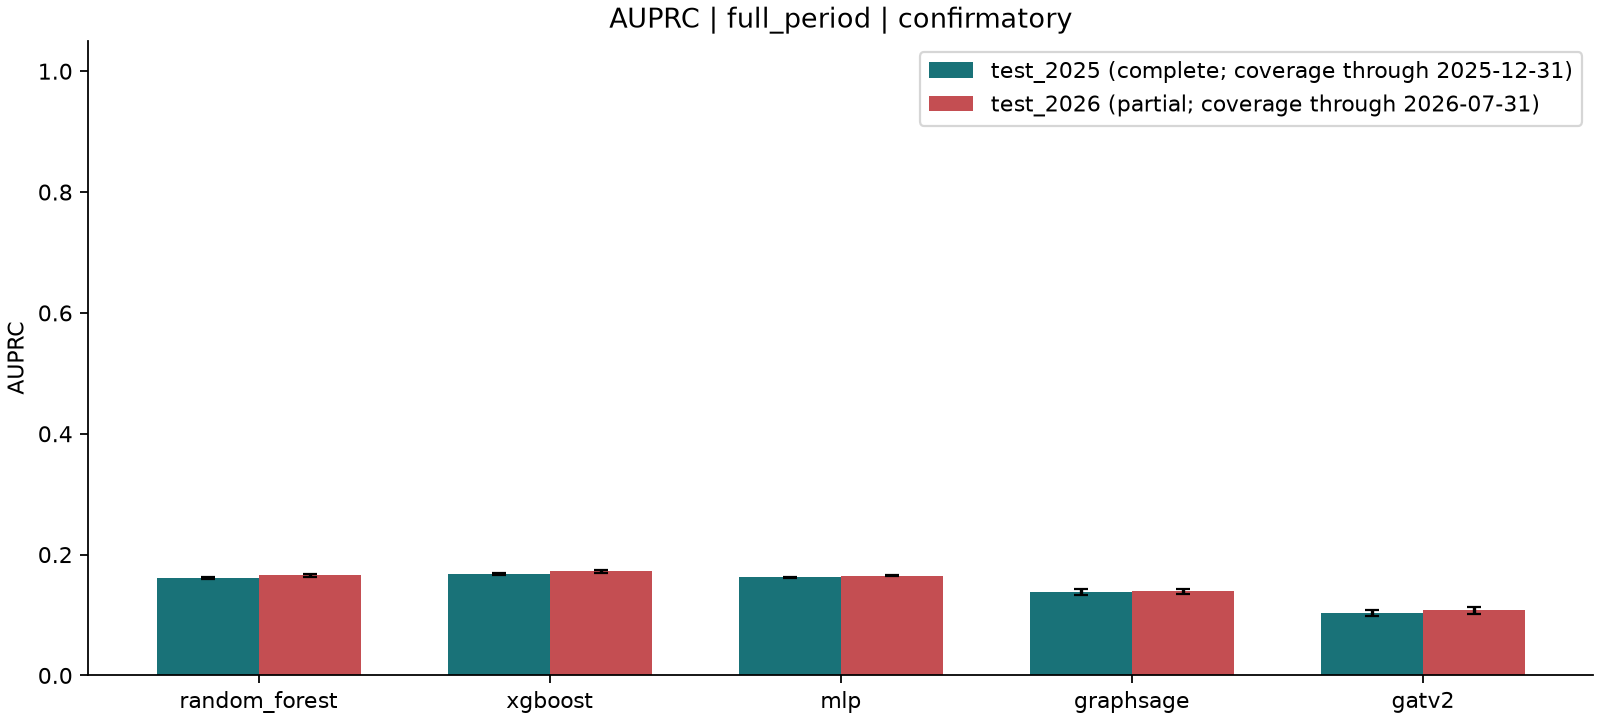
\includegraphics[width=0.92\textwidth]{imagens/auprc-full_period.png}
\caption{AP dos cinco modelos nos períodos completos de avaliação. As
barras de erro representam um desvio-padrão entre sementes. O teste de
2026 é parcial.}
\label{fig:ap-modelos}
\end{figure}

As métricas dependentes de limiar mostram compromissos distintos. Em
2025, Random Forest obteve a maior precisão média (19,99\%) e o maior
F1 (24,86\%), enquanto MLP obteve a maior revocação (36,33\%). XGBoost
combinou precisão de 19,39\% e revocação de 35,74\%. Em 2026, Random
Forest manteve a maior precisão (20,47\%), MLP a maior revocação
(37,85\%) e XGBoost o maior F1 por pequena margem (24,84\%). Portanto,
a liderança de XGBoost em AP não implica domínio em todos os pontos de
operação.

AUROC acima de 90\% nos quatro melhores modelos pode parecer elevada,
mas não elimina a dificuldade da classe rara. Mesmo com ordenação útil,
as precisões próximas de 20\% indicam aproximadamente quatro falsos
positivos para cada verdadeiro positivo entre as unidades sinalizadas
nos limiares congelados. As revocações médias variaram de 23,87\% a
37,85\% entre os cinco modelos nos dois testes, indicando que cada
modelo, isoladamente, deixou de identificar a maioria das unidades
positivas. Acurácia seria enganosa: sempre prever ausência já produziria
98,55\% em 2025 e 98,58\% em 2026, com revocação zero.

O teste de 2026 reutilizou os modelos sem ajuste e apresentou ranking
semelhante ao de 2025. Na comparação sazonal restrita às mesmas semanas
ISO, a AP do XGBoost passou de 15,89\% em 2025 para 17,23\% em 2026;
os demais modelos também tiveram AP maior em 2026. Esse resultado é
descritivo e não demonstra tendência anual: diferenças de tráfego,
registro, cobertura ou condições externas não foram controladas.

\subsection{A topologia melhorou a predição?}

A resposta depende da arquitetura, mas não foi suficiente para superar
as referências tabulares. No GraphSAGE, remover a passagem de mensagens
reduziu a AP de 13,86\% para 13,26\%, diferença emparelhada de
$+0,60\pp$ a favor do modelo completo. A AUROC caiu 0,25\pp, enquanto
o F1 permaneceu praticamente igual. Há, portanto, evidência descritiva
de um pequeno sinal topológico para o GraphSAGE neste protocolo.

No GATv2 ocorreu o inverso: a variante sem topologia atingiu AP de
13,70\%, contra 10,37\% do modelo completo, diferença de
$-3,33\pp$. AUROC, F1, precisão e revocação também melhoraram sem
mensagens de vizinhos. Sob cinco épocas e a configuração adotada, a
agregação por atenção esteve associada a menor desempenho. Entre as
possíveis explicações estão otimização insuficiente, heterogeneidade
das vizinhanças, ruído estrutural e ausência de atributos que tornem a
relação entre segmentos informativa. Essas hipóteses não foram isoladas
neste experimento.

\begin{table}[htbp]
\centering
\caption{Ablações das GNNs em 2025. AP média em porcentagem e diferença
do modelo completo para a variante.}
\label{tab:ablacoes}
\small
\setlength{\tabcolsep}{5pt}
\begin{tabular}{llrr}
\toprule
\textbf{Modelo} & \textbf{Variante} & \textbf{AP} &
\textbf{Completo $-$ variante} \\
\midrule
\multirow{4}{*}{GraphSAGE}
& Completo & 13,86 & --- \\
& Sem atributos viários & 1,51 & $+12,35\pp$ \\
& Sem atributos temporais & 14,36 & $-0,51\pp$ \\
& Sem topologia & 13,26 & $+0,60\pp$ \\
\midrule
\multirow{4}{*}{GATv2}
& Completo & 10,37 & --- \\
& Sem atributos viários & 1,49 & $+8,88\pp$ \\
& Sem atributos temporais & 10,87 & $-0,50\pp$ \\
& Sem topologia & 13,70 & $-3,33\pp$ \\
\bottomrule
\end{tabular}
\end{table}

Os atributos de via foram decisivos: sua remoção levou a AP para 1,51\%
no GraphSAGE e 1,49\% no GATv2, valores próximos da prevalência. O alto
\textit{recall} dessas variantes não representa bom desempenho, pois
foi acompanhado de precisão próxima de 1,5\%. Já remover os atributos
temporais aumentou ligeiramente a AP média das duas GNNs. Como os
históricos estavam ausentes por falta de prova de disponibilidade, a
variante remove essencialmente o calendário. O resultado não prova que
sazonalidade seja irrelevante; indica apenas que essas codificações não
acrescentaram AP com o orçamento atual.

\subsection{Custo computacional}

XGBoost apresentou simultaneamente a maior AP e o menor tempo médio de
ajuste entre os modelos completos: 75,2 segundos. GraphSAGE treinou em
118,0 segundos, enquanto MLP e GATv2 demandaram 272,0 e 450,8 segundos.
Random Forest ocupou o maior artefato de modelo (31,78 MiB), embora os
picos de memória total tenham sido dominados pela carga dos dados e das
bibliotecas, entre 5,7 e 6,2 GiB.

\begin{table}[htbp]
\centering
\caption{Custo médio dos modelos completos em CPU. Inferência inclui
carregamento, verificação e pré-processamento; RSS é o maior pico
amostrado entre sementes.}
\label{tab:custos}
\footnotesize
\setlength{\tabcolsep}{4pt}
\begin{tabular}{lrrrr}
\toprule
\textbf{Modelo} & \textbf{Treino (s)} & \textbf{Inf. 2025 (s)} &
\textbf{Inf. 2026 (s)} & \textbf{RSS (MiB)} \\
\midrule
Random Forest & 154,85 & 5,60 & 3,09 & 5.874,49 \\
XGBoost & 75,20 & 2,58 & 1,53 & 6.001,33 \\
MLP & 271,99 & 5,53 & 0,67 & 6.139,52 \\
GraphSAGE & 117,96 & 6,40 & 84,90 & 6.303,03 \\
GATv2 & 450,83 & 10,96 & 6,65 & 6.059,39 \\
\bottomrule
\end{tabular}
\end{table}

O tempo de inferência do GraphSAGE em 2026 foi anormalmente maior que
em 2025 apesar do conjunto menor, sinal de que carga concorrente,
caches e custos de inicialização influenciaram a medição. Por isso, os
tempos caracterizam as execuções registradas e não devem ser tratados
como comparação isolada de complexidade algorítmica. Ainda assim, o
GATv2 foi consistentemente o modelo mais caro para treinar e obteve o
menor desempenho.

\subsection{Relação com a literatura, limitações e reprodução}

Em relação a Araújo \cite{araujo2022}, o trabalho acrescenta uma tarefa
preditiva com separação temporal e representação explícita da malha,
mas não compara AP ou AUROC com regras de associação. Em relação a
Amorim et al. \cite{amorim2023}, a acurácia alta deste estudo não pode
ser interpretada como superioridade, pois o alvo e a população são
distintos e a classe negativa domina as observações. Comparado ao valor
de AUROC de 90,1\% de Zhang et al. \cite{zhang2026}, XGBoost e
GraphSAGE ficaram numericamente próximos ou acima, mas sem equivalência
de dados, tarefa ou modalidades. O resultado interno mais sólido é que
os modelos tabulares superaram as GNNs em AP.

As conclusões possuem seis limitações principais. Primeiro, a cobertura
temporal foi assumida, não comprovada documentalmente; registros
faltantes podem criar falsos negativos. Segundo, a rede é estática e
anterior a 2019, podendo omitir alterações posteriores e trechos que
cruzam a fronteira estadual. Terceiro, não há denominador de volume de
tráfego, de modo que o alvo representa ocorrência registrada, não taxa
de risco ajustada à exposição. Quarto, históricos de acidentes ficaram
ausentes por falta de prova de publicação anterior. Quinto, redes
neurais foram treinadas por apenas cinco épocas, com um candidato por
variante, sem demonstração de convergência. Sexto, ambos os testes usam
a mesma geografia; não foi avaliada generalização para outros estados.

As diferenças entre médias e ablações são descritivas, não testes de
significância ou de causalidade. A reutilização de 2025 e 2026 para uma
nova busca de hiperparâmetros exigiria outro protocolo, pois esses
testes já foram observados.

Por outro lado, a integridade computacional foi verificada. O pacote
final reconstruiu o conjunto de dados e repetiu todas as inferências
dos modelos completos em processo separado, sem rede e sem chamadas de
treinamento. A diferença máxima nas métricas foi 0,0\pp e os motivos de
métricas indefinidas foram preservados. A reprodução ocorreu no mesmo
ambiente de bibliotecas; portanto, confirma rastreabilidade e repetição
local, mas não substitui uma replicação independente.

% ============================================================
% Conclusão: máximo de meia página de texto
% ============================================================
\section{Conclusão}
\label{sec:conclusao}

Este trabalho avaliou se a conectividade da malha federal de Minas
Gerais melhora a predição semanal de acidentes registrados pela PRF.
Foi construída uma base com 10.973 segmentos, mais de 4,3 milhões de
unidades segmento--semana e cinco famílias de modelos avaliadas em
períodos posteriores ao treinamento. XGBoost obteve a maior AP em 2025
(16,75\%) e em 2026 parcial (17,23\%). GraphSAGE e GATv2 não superaram
os modelos tabulares. A topologia produziu pequeno ganho de AP no
GraphSAGE e perda no GATv2, mostrando que passagem de mensagens não é
automaticamente benéfica. As ablações indicaram que os atributos da via
foram a principal fonte de sinal preditivo.

A contribuição central é uma comparação brasileira, temporalmente
separada, auditável e reproduzível, inclusive quando o resultado não
confirma a superioridade esperada das GNNs. As conclusões permanecem
condicionadas à cobertura assumida dos arquivos, à malha histórica, à
ausência de exposição ao tráfego e ao orçamento restrito. Estudos
posteriores devem obter evidência documental de cobertura e
disponibilidade, incorporar volume de tráfego e mudanças da rede, e
avaliar novas configurações em um protocolo que reconheça que os testes
atuais já foram observados.

% ============================================================
% Referências: extensão livre
% ============================================================
\bibliographystyle{sbc}

\begin{thebibliography}{99}

\bibitem{who2023}
World Health Organization.
\newblock \textit{Global Status Report on Road Safety 2023}.
\newblock Geneva: WHO, 2023.
\newblock Disponível em:
\url{https://www.who.int/publications/i/item/9789240086517}.

\bibitem{prf2026}
Polícia Rodoviária Federal.
\newblock Balanço da PRF mostra redução da letalidade nas BRs em 2025.
\newblock Governo Federal, fev. 2026.
\newblock Disponível em:
\url{https://www.gov.br/prf/pt-br/noticias/nacionais/2026/fevereiro/menos-mortes-e-feridos-balanco-da-prf-mostra-reducao-da-letalidade-nas-brs-em-2025}.

\bibitem{araujo2022}
R. B. de Araújo.
\newblock \textit{Regras de associação entre as características dos
veículos e os acidentes de trânsito em rodovias federais brasileiras
por meio de aprendizado de máquina}.
\newblock Dissertação de Mestrado, Universidade Federal de Minas
Gerais, 2022.
\newblock Disponível em:
\url{https://repositorio.ufmg.br/items/829406e3-546d-438c-88ce-d22fc18bba88}.

\bibitem{amorim2023}
B. de S. P. Amorim, A. A. Firmino, G. Braz Júnior et al.
\newblock A Machine Learning Approach for Classifying Road Accident
Hotspots.
\newblock \textit{ISPRS International Journal of Geo-Information},
v. 12, n. 6, art. 227, 2023.
\newblock Disponível em:
\url{https://www.mdpi.com/2220-9964/12/6/227}.

\bibitem{nippani2023}
A. Nippani, D. Li, H. Ju, H. N. Koutsopoulos e H. Zhang.
\newblock Graph Neural Networks for Road Safety Modeling: Datasets and
Evaluations for Accident Analysis.
\newblock In: \textit{NeurIPS 2023 Datasets and Benchmarks}, 2023.
\newblock Disponível em:
\url{https://proceedings.neurips.cc/paper_files/paper/2023/hash/a365be0950259c9624edfb4d26eabd46-Abstract-Datasets_and_Benchmarks.html}.

\bibitem{zhang2026}
Z. Zhang, M. Duan, H. N. Koutsopoulos e H. R. Zhang.
\newblock Learning Multimodal Embeddings for Traffic Accident
Prediction and Causal Estimation.
\newblock In: \textit{Proceedings of KDD}, 2026.
\newblock Disponível em:
\url{https://arxiv.org/abs/2512.02920}.

\bibitem{zhuang2024}
X. Gao, X. Jiang, D. Zhuang, H. Chen, S. Wang, S. Law e J. Haworth.
\newblock Uncertainty-Aware Probabilistic Graph Neural Networks for
Road-Level Traffic Accident Prediction.
\newblock \textit{arXiv:2309.05072v4}, 2024.
\newblock Disponível em:
\url{https://arxiv.org/abs/2309.05072}.

\bibitem{breiman2001}
L. Breiman.
\newblock Random Forests.
\newblock \textit{Machine Learning}, v. 45, n. 1, p. 5--32, 2001.
\newblock DOI: \url{https://doi.org/10.1023/A:1010933404324}.

\bibitem{chen2016}
T. Chen e C. Guestrin.
\newblock XGBoost: A Scalable Tree Boosting System.
\newblock In: \textit{Proceedings of KDD}, p. 785--794, 2016.
\newblock Disponível em:
\url{https://arxiv.org/abs/1603.02754}.

\bibitem{goodfellow2016}
I. Goodfellow, Y. Bengio e A. Courville.
\newblock \textit{Deep Learning}.
\newblock Cambridge: MIT Press, 2016.
\newblock Disponível em: \url{https://www.deeplearningbook.org/}.

\bibitem{hamilton2017}
W. L. Hamilton, R. Ying e J. Leskovec.
\newblock Inductive Representation Learning on Large Graphs.
\newblock In: \textit{NeurIPS}, p. 1024--1034, 2017.
\newblock Disponível em:
\url{https://arxiv.org/abs/1706.02216}.

\bibitem{brody2022}
S. Brody, U. Alon e E. Yahav.
\newblock How Attentive are Graph Attention Networks?
\newblock In: \textit{ICLR}, 2022.
\newblock Disponível em:
\url{https://arxiv.org/abs/2105.14491}.

\bibitem{saito2015}
T. Saito e M. Rehmsmeier.
\newblock The Precision-Recall Plot Is More Informative than the ROC
Plot When Evaluating Binary Classifiers on Imbalanced Datasets.
\newblock \textit{PLOS ONE}, v. 10, n. 3, e0118432, 2015.
\newblock DOI: \url{https://doi.org/10.1371/journal.pone.0118432}.

\end{thebibliography}

\end{document}